\documentclass[
 openright,
 %twoside, % beidseitig für Druck
 a4paper
]{scrreprt}
%scrreprt
%% HTW Dresden Corporate Design
%% Copyright (C) Falk-Jonatan Strube <falkjonatanstrube@gmail.com>, 2017
%%% === Anfang Paket htwscr ===
\makeatletter
\ifcsname KOMAoption\endcsname%
%\KOMAoption{footheight}{11mm}	% mehr Platz für Wasserzeichen o.ä. in der Fußzeile
\recalctypearea	% s.o.
\RequirePackage{geometry}
\geometry{
	top=25mm, 
	bottom=25mm, 
	%headsep=10mm, 
	inner=25mm, 
	outer=25mm, 
	%footskip=15mm, 
	marginparsep=2mm
}
\RequirePackage{helvet}	% Corporate Design schreibt Arial/Helvetica vor
\renewcommand{\familydefault}{\sfdefault}	% s.o.
\RequirePackage{graphicx}	% für Grafiken
\RequirePackage{xcolor}		% für Farben
\definecolor{htworange}{RGB}{249,155,28}	% Corporate Design orange CMYK(0/45/100/0)
\definecolor{htwblue}{RGB}{0,116,188}			% Corporate Design blau CMYK(90/50/0/0)
\definecolor{htwgrey}{RGB}{128,128,128}		% Corporate Design gray 60% Schwarz [Annahme: CMYK(0,0,0,60)]
\RequirePackage{ifthen,xifthen}	% für Bedingungen/Optionen
\RequirePackage{etoolbox}				% s.o.

%%% Format des HTW-Headers (wird hier als Texteelement verwenden) nach dem Style der PowerPoint-Vorlagen. Weiterhin inspiriert durch das Paket tudscr (Corporate Design der TU Dresden)
%%% Dateipfad des Logos abhängig von der Verwendung als Paket/Input
\ifdefined\@isHTWCDpackage%
	\gdef\@pathtoimage{HTW}%
\else%
	\ifdefined\pathtomaster%
		\gdef\@pathtoimage{\pathtomaster /HTW}%
	\else 
		\gdef\@pathtoimage{htwcd/HTW}%
	\fi%
\fi%
\newcommand{\pathtologo}[1]{\gdef\@pathtoimage{#1}}
%%% Berechnung der Größe des Logos
\newlength{\htwLogoHeight}
\setlength{\htwLogoHeight}{12mm}	% Mindesthöhe des Logos laut Corporate Design: 11mm
\newlength{\@htwLogoWidth}
\AtBeginDocument{
\def\printLogo{\includegraphics[height=\htwLogoHeight]{\@pathtoimage}}
\setlength\@htwLogoWidth{\widthof{\printLogo}}
}
%%% Definition des Header
\newcommand{\@htwheader}{{\noindent%
%%% Header ist abhängig von dem Vorhandensein von department, institute und chair
\newcommand{\hasDepInsCh}{\gdef\@hasDepInsCh{}}%
\ifdefined\@department\hasDepInsCh\fi%
\ifdefined\@institute\hasDepInsCh\fi%
\ifdefined\@chair\hasDepInsCh\fi%
\begin{minipage}[b][\htwLogoHeight]{\dimexpr \textwidth - \@htwLogoWidth - 2mm \relax}% 2mm Abstand zwischen Logo und Linie
{\small{\bfseries%
\ifdefined\@faculty\@faculty{}\fi} %
\strut}%
{\color{htworange}\hrule height 1pt}%
\vspace{.1mm}%
\end{minipage}
\hfill%
\begin{minipage}[b][\htwLogoHeight]{\@htwLogoWidth}
\includegraphics[height=\htwLogoHeight]{\@pathtoimage}
\end{minipage}
\ifdefined\@hasDepInsCh%
\\%
\begin{minipage}{\textwidth}
\small%
\ifdefined\@department\@department{}\fi%
\ifdefined\@institute\ifdefined\@department,~\fi \@institute\fi%
\ifdefined\@chair\ifdefined\@department,~\else\ifdefined\@institute,~\fi\fi\@chair\fi\strut
%{\color{htworange}\hrule height 0.5pt}
\end{minipage}
\fi
}}

%%% Definition der Fußzeilen
\usepackage{scrlayer-scrpage}
\@ifclassloaded{scrreprt}{%
\renewcommand*{\partpagestyle}{scrheadings}
\renewcommand*{\chapterpagestyle}{scrheadings}%
}{}
\pagestyle{scrheadings}
% Definition der Seitenzahl-Position:

%\newif \if@twoside \@twosidefalse
%\if@twoside%
	%
%\else%
	% Beim einseitigen Dokument Seitenzahl auch außen/rechts.
%	\ofoot{\pagemark}%
%	\cfoot{}%
%\fi%  

%%% Einstellungen
\newcommand{\simpledate}{\gdef\@simpledate{}}		% Datum nicht mit "Eingereicht am:" Vorsatz
\newcommand{\nouppercase}{\gdef\@nouppercase{}}	% Titel/Parts/Chapters usw. nicht in Großbuchstaben

%%% Einiges erst zu Beginn des Dokumentes ausführen, um Einstellungen zu berücksichtigen
\AtBeginDocument{
\renewcommand\SS{SS}	% fix big ß
%%% Sektionen usw. ggf. in Großbuchstaben:
\providecommand{\chapterlinesformat}[3]{}	% compatibility
\providecommand{\chapterlineswithprefixformat}[3]{}	% compatibility
\providecommand{\sectionlinesformat}[4]{}	% compatibility
\ifdefined\@nouppercase\relax\else
\renewcommand\sectionlinesformat[4]{\@hangfrom{\hskip#2 #3}{\MakeUppercase{#4}}}
\@ifclassloaded{scrreprt}{%
\renewcommand\chapterlinesformat[3]{\@hangfrom{#2}{\MakeUppercase{#3}}}
\renewcommand\chapterlineswithprefixformat[3]{\MakeUppercase{#2#3}}%
}{}
\fi
%%% Anpassung der Part-Seite
\renewcommand*{\partheadstartvskip}{\@htwheader\vspace*{30mm}}
\renewcommand*{\raggedpart}{\raggedright}
\renewcommand*{\partformat}{\huge\ifdefined\@nouppercase \partname~\thepart\else\MakeUppercase{\partname~\thepart}\fi.}
\ifdefined\@nouppercase\setkomafont{part}{\Huge}\else\setkomafont{part}{\Huge\MakeUppercase}\fi
}

\newcommand{\bilingual}[3]{\ifdefined #1 \let #1\undefined\fi\newcommand{#1}{\iflanguage{english}{#3}{#2}}}	% Übersetzung von einigen Variablen in mehrere Sprachen

\newcommand{\checkThesis}[2]{\ifthenelse{\equal{#1}{diss}\OR\equal{#1}{doctoral}\OR\equal{#1}{phd}}{
\gdef#2{\dissertationname}}{
\ifthenelse{\equal{#1}{diploma}}{
\gdef#2{\diplomathesisname}}{
\ifthenelse{\equal{#1}{master}}{
\gdef#2{\masterthesisname}}{
\ifthenelse{\equal{#1}{bachelor}}{
\gdef#2{\bachelorthesisname}}{
\ifthenelse{\equal{#1}{student}}{
\gdef#2{\studentthesisname}}{
\ifthenelse{\equal{#1}{evidence}}{
\gdef#2{\studentresearchname}}{
\ifthenelse{\equal{#1}{project}}{
\gdef#2{\projectpapername}}{
\ifthenelse{\equal{#1}{seminar}}{
\gdef#2{\seminarpapername}}{
\ifthenelse{\equal{#1}{term}}{
\gdef#2{\termpapername}}{
\ifthenelse{\equal{#1}{research}}{
\gdef#2{\researchname}}{
\ifthenelse{\equal{#1}{log}}{
\gdef#2{\logname}}{
\ifthenelse{\equal{#1}{report}}{
\gdef#2{\reportname}}{
\ifthenelse{\equal{#1}{internship}}{
\gdef#2{\internshipname}}{
\ifthenelse{\equal{#1}{lecture}\OR\equal{#1}{lesson}\OR\equal{#1}{pract}}{
\bilingual{\professorname}{Vorlesung von}{Lecture by}
\simpledate
\gdef\@islecture{\relax}
\ifthenelse{\equal{#1}{lecture}}{\gdef#2{\lecturename}}{
\ifthenelse{\equal{#1}{lesson}}{\gdef#2{\lessonname}}{
\gdef#2{\practname}
}}}{
\gdef#2{#1}}}}}}}}}}}}}}}}

%%% Textfragmente der Titelseite in deutsch und englisch
\bilingual{\dateofbirthname}{Geboren am:}{Born on:}
\bilingual{\placeofbirthname}{in}{in}
\bilingual{\coursename}{Studiengang:}{Course:}
\bilingual{\disciplinename}{Studienrichtung:}{Discipline:}
\bilingual{\matriculationnumbername}{Matrikelnummer:}{Matriculation number:}
\bilingual{\matriculationyearname}{Immatrikulationsjahr}{Matriculation year:}
\bilingual{\graduationname}{zur Erlangung des akademischen Grades}{to achieve the academic degree}
\bilingual{\refereename}{Gutachter}{Referee}
\bilingual{\advisorname}{Fachreferent}{Advisor}
\bilingual{\supervisorname}{Betreuer}{Supervisor}
\bilingual{\professorname}{Betreuender Hochschullehrer}{Supervising professor}
\bilingual{\datename}{Eingereicht am:}{Submitted on:}
%% Thesis Typen (inspiriert von dem Paket tudscr):
\bilingual{\dissertationname}{Dissertation}{Dissertation} % diss, doctoral, phd 
\bilingual{\diplomathesisname}{Diplomarbeit}{Diploma Thesis} % diploma 
\bilingual{\masterthesisname}{Master-Arbeit}{Master Thesis} % master 
\bilingual{\bachelorthesisname}{Bachelor-Arbeit}{Bachelor Thesis} % bachelor 
\bilingual{\studentthesisname}{Studienarbeit}{Student Thesis} % student 
\bilingual{\studentresearchname}{Großer Beleg}{Student Research Project} % evidence 
\bilingual{\projectpapername}{Projektarbeit}{Project Paper} % project
\bilingual{\seminarpapername}{Seminararbeit}{Seminar Paper} % seminar
\bilingual{\termpapername}{Hausarbeit}{Term Paper} % term
\bilingual{\researchname}{Forschungsbericht}{Research Report} % research 
\bilingual{\logname}{Protokoll}{Log} % log 
\bilingual{\reportname}{Bericht}{Report} % report
\bilingual{\internshipname}{Praktikumsbericht}{Internship Report} % internship 
\bilingual{\lecturename}{Vorlesungsmitschrift}{Lecture Notes} % lecture 
\bilingual{\lectureauthorname}{Mitschrift von}{Notes by} % lecture  
\bilingual{\lessonname}{\"Ubungsmitschrift}{Lesson Notes} % lecture  
\bilingual{\practname}{Praktikumsmitschrift}{Pracital Course Notes} % lecture 
%%% Variablen für die Titelseite (inspiriert von dem Paket tudscr):
\renewcommand{\subject}[1]{\checkThesis{#1}{\@subject}}
\newcommand{\faculty}[1]{\gdef\@faculty{#1}}
\newcommand{\department}[1]{\gdef\@department{#1}}
\newcommand{\institute}[1]{\gdef\@institute{#1}}
\newcommand{\chair}[1]{\gdef\@chair{#1}}
\newcommand{\authormore}[1]{\gdef\@authormore{#1}}
\newcommand{\dateofbirth}[1]{\gdef\@dateofbirth{#1}}
\newcommand{\placeofbirth}[1]{\gdef\@placeofbirth{#1}}
\newcommand{\course}[1]{\gdef\@course{#1}}
\newcommand{\discipline}[1]{\gdef\@discipline{#1}}
\newcommand{\matriculationnumber}[1]{\gdef\@matriculationnumber{#1}}
\newcommand{\matriculationyear}[1]{\gdef\@matriculationyear{#1}}
\newcommand{\thesis}[1]{\checkThesis{#1}{\@thesis}}
\newcommand{\graduation}[2][]{\gdef\@graduation{#2}\gdef\@graduationshort{#1}}
\newcommand{\supervisor}[1]{\gdef\@supervisor{#1}}
\newcommand{\referee}[1]{\gdef\@referee{#1}}
\newcommand{\advisor}[1]{\gdef\@advisor{#1}}
\newcommand{\professor}[1]{\gdef\@professor{#1}}
%%% Titelseite (inspiriert von dem Paket tudscr):
\renewcommand*{\maketitle}{%
\begin{titlepage}%
\begin{flushleft}
\renewcommand{\thefootnote}{$\star$}%
%%% Kopfzeile HTW-Style:
\@htwheader\\[13mm]
%%% Die Zeilen für titlehead, subject, title, subtitle und author sind immer vorhanden (spacing)
{\noindent\@titlehead{}\strut}\\[3mm]%
{\Large\@subject{}\strut}\\[8mm]%
{\Huge\bfseries%
\ifdefined\@nouppercase\@title{}\else\MakeUppercase{\@title{}}\fi%
\strut}\\
{\Large\bfseries%
\ifdefined\@nouppercase\@subtitle{}\else\MakeUppercase{\@subtitle{}}\fi%
\strut}\\[11mm]
\ifdefined\@islecture\strut\else{\Large\@author{}\strut}\fi % Autor wird bei Vorlesungsmitschrift unten angezeigt
%%% Weitere Felder werden nur angezeigt, wenn sie definiert wurden
\ifdefined\@authormore\ifdefined\@islecture\else\\\fi{\@authormore{}\strut}\fi
\ifdefined\@dateofbirth\\\dateofbirthname{} \@dateofbirth{} \ifdefined\@placeofbirth\placeofbirthname{} \@placeofbirth{}\strut\fi\fi
\ifdefined\@course\\\coursename{} \@course{}\strut\fi
\ifdefined\@discipline\\\disciplinename{} \@discipline{}\strut\fi
\ifdefined\@matriculationnumber\\\matriculationnumbername{} \@matriculationnumber{}\strut\fi
\ifdefined\@matriculationyear\\\matriculationyearname{} \@matriculationyear{}\strut\fi
\ifdefined\@thesis\\[10mm]{\LARGE\bfseries
\ifdefined\@nouppercase\@thesis{}\else\MakeUppercase{\@thesis{}}\fi
\strut}
\ifdefined\@graduation\\[2mm]{\graduationname{}\strut}
\\[5mm]{\LARGE\bfseries
\ifdefined\@nouppercase\relax\else\MakeUppercase{\fi%
\@graduation{} \ifdefined\@graduationshort(\@graduationshort{})\fi
\ifdefined\@nouppercase\relax\else}\fi\strut}\fi\fi
\vfill\noindent
\ifdefined\@islecture\\[1mm]{\lectureauthorname{}\strut}\\[.7mm]{\Large\@author{}\strut}\fi
\ifdefined\@referee{\refereename{}\strut}\\[.7mm]{\Large\@referee{}\strut}\fi
\ifdefined\@advisor\\[1mm]{\advisorname{}\strut}\\[.7mm]{\Large\@advisor{}\strut}\fi
\ifdefined\@supervisor\\[1mm]{\supervisorname{}\strut}\\[.7mm]{\Large\@supervisor{}\strut}\fi
\ifdefined\@professor\\[1mm]{\professorname{}\strut}\\[.7mm]{\Large\@professor{}\strut}\fi
\ifdefempty{\@date}{}{\ifdefined\@simpledate\\[6mm]\relax\else\\[3mm]\datename{}~\fi\@date{}\strut}
\ifdefempty{\@publishers}{}{\\[4.5mm]{\Large\@publishers{}\strut}}%
\renewcommand\footnoterule{}
\@thanks\global\let\@thanks\@empty
\end{flushleft}
\end{titlepage}
\setcounter{footnote}{0}
}
\else%
\PackageError{htwcd}{htwcd needs a KOMA class!}%
\fi%
\makeatother
%%% === Ende Paket htwscr ===

% Vorgaben zum Seitenrand	
\geometry{
	top=30mm, 
	bottom=30mm, 
	%headsep=15mm, 
	inner=40mm, 
	outer=20mm, 
	%left=40mm,
	%right=20mm,
	%footskip=15mm,
}

\usepackage{scrlayer-scrpage}
\pagestyle{scrheadings}
\clearpairofpagestyles
\ofoot{\pagemark}
\raggedbottom

% Codierung
\usepackage[utf8]{inputenc}
\usepackage[T1]{fontenc}
\usepackage[ngerman]{babel}
\usepackage{csquotes}	% Anführungszeichen
\usepackage{amssymb}

% Grafiken
\usepackage{graphicx}
\graphicspath{ {./images/} }
\usepackage{float}
\usepackage{longtable}

% Quelltext
\usepackage{listings}
\usepackage{scrhack}

% Links
\usepackage{xurl}
\usepackage[bookmarks,%
bookmarksopen=false,% Klappt die Bookmarks in Acrobat aus
colorlinks=true,%
linkcolor=black,%
citecolor=black,%
urlcolor=black,%
]{hyperref}

\usepackage{datetime}


\usepackage{tikz}
\usetikzlibrary{positioning,shadings}
\usetikzlibrary{arrows}

% ======================================================
% Informationen für das Dokument und Titelseite:
% ======================================================
\faculty{Fakultät Informatik/Mathematik}

\title{Persönliche Daten in der Datenökonomie}

\author{
	Maria Mukian\\
	Philipp Steigler\\
	Eric Hans Gero Biele
}

\professor{Prof. Dr. Jürgen Anke}

\newdate{abgabe}{26}{01}{2021}
\date{\displaydate{abgabe}}
% ======================================================


% ======================================================
% Literatur/Quellen und Akronyme/Glossar:
% ======================================================
\usepackage[
backend=bibtex,
sortlocale=de_DE, 
bibencoding=utf8,
style=numeric, 
citestyle=numeric,
doi=false,
isbn=false,
url=false,
sorting=nty
]{biblatex}	% BibTeX
\bibliography{Bibliography}

\usepackage[acronym]{glossaries}
\makeglossaries
% ------------------------------------------
% Glossar  
% keine Umlaute im entry verwenden   
\newglossaryentry{natuerlichePersonG}
{
name={natürliche Person},
description={\glqq Eine natürliche Person meint den Menschen als Rechtssubjekt und somit als Träger von Rechten und Pflichten.\grqq{} \cite{NatPerson_2018}}
}

\newglossaryentry{webScrapingG}
{
name={Web-Scraping},
description={\glqq Web-Scraping ist das Schürfen von Daten, also die Datenextraktion aus Webseiten.\grqq{} \cite{webScraping_2021}}
}

\newglossaryentry{brokerG}
{
name={Broker},
description={\glqq Der Broker wirkt als Makler bei reiner Geschäftsvermittlung auf fremden Namen und auf fremde Rechnung (Abschlussvermittlung) oder als Kommissionär in eigenem Namen und auf fremde Rechnung.\grqq{} \cite{broker_2018}}
}

\newglossaryentry{smartContractsG}
{
name={Smart Contract},
description={\glqq Smart Contracts sind digitale Verträge, die in einer Blockchain gespeichert sind und automatisch ausgeführt werden, wenn vordefinierte Bedingungen erfüllt sind\grqq{} \cite{smartContract_2022}}
}

%============================================
% Akronyme
%============================================
\newglossaryentry{DSGVO}{
	type=\acronymtype, 
	name={DSGVO}, 
	description={Datenschutz-Grundverordnung}
}

\newglossaryentry{UN}{
	type=\acronymtype, 
	name={UN}, 
	description={United Nations}
}

\newglossaryentry{SaaS}{
	type=\acronymtype, 
	name={SaaS}, 
	description={Software as a Service}
}

\newglossaryentry{PaaS}{
	type=\acronymtype, 
	name={PaaS}, 
	description={Platform as a Service}
}
% ======================================================
\pagenumbering{roman}

\begin{document}
% ==============================================
% Deckblatt
% ==============================================
\maketitle

% ==============================================
% Abstract
% ==============================================
\setcounter{page}{1}
\pagenumbering{gobble}
\thispagestyle{empty}
\vspace*{5cm}
\begin{center}
\begin{minipage}{0.9\textwidth}
\chapter*{Abstract}

Die vorliegende Arbeit gibt einen Überblick über die Möglichkeiten der aktiven Monetarisierung von persönlichen Daten mit deren Potenzial und Einschränkungen. Im Zuge dessen wurden die Grundlagen der Datenökonomie, sowie der monetäre Wert von Daten untersucht und darauf aufbauend eine Fallstudie durchgeführt, welche die Basis dieser Arbeit bildet. Die Ergebnisse der Fallstudie führten zu einer Kategorisierung der Monetarisierungsmöglichkeiten durch den Verbraucher. Diese Arbeit ist sowohl für IT- und Wirtschaftswissenschaftler, als auch für Unternehmen und Verbraucher selbst interessant, die sich auf datengetriebene Technologien stützen.

\vspace*{1.5cm}
\end{minipage}
\end{center}
\clearpage

% ==============================================
% Verzeichnisse:
% ==============================================
% Inhaltsverzeichnis
\pagenumbering{roman}
\setcounter{page}{1}
\tableofcontents
% Abkürzungsverzeichnis
% ACHTUNG: Akronyme und Glossar muss (ähnlich wie bibtex) extra kompiliert werden über makeglossaries (in texmaker bspw. "makeglossaries %")
\printglossary[type=\acronymtype]
\addcontentsline{toc}{chapter}{Akronyme}
% Glossar
\printglossary[type=main]
\addcontentsline{toc}{chapter}{Glossar}
% Abbildungsverzeichnis
\listoffigures
\addcontentsline{toc}{chapter}{Abbildungsverzeichnis}
% Tabellenverzeichnis
\listoftables
\addcontentsline{toc}{chapter}{Tabellenverzeichnis}

% ==============================================
% Textteil
% Richtlinie: 25-40 Seiten
% \section{}, \subsection{}, \subsubsection{}
% ==============================================
\clearpage
\pagenumbering{arabic}
\chapter{Einleitung}
% * Einleitung
\section{Motivation}\label{Motivation}
Die Verbreitung des Internets auf Computern und mobilen Endgeräten hat zu einer Produktion riesiger Datenmengen geführt. Diese Daten -- insbesondere personenbezogene Daten -- haben sich zu einer wichtigen Ressource entwickelt, mit der Unternehmen einen Mehrwert erzeugen. Im Weiteren entstand daraus eine Datenökonomie, die allein auf dem Handel und der Verarbeitung personenbezogener Daten beruhen. \cite{humanDemand_2020} Dabei werden Daten meist jedoch nicht direkt von den Erzeugern, den individuellen Personen, verkauft. Stattdessen erheben große Internetdienste Anspruch auf die Daten ihrer Nutzer durch Klauseln in den Nutzungsbedingungen und verkaufen diese dann an Dritte weiter -- oftmals ohne Nutzer im Einzelfall darüber in Kenntnis zu setzen. Obwohl Individuen durch Erzeugung von Daten die Grundlage solcher Ökosysteme bilden, werden sie von Unternehmen bislang nur als Datenquelle gesehen und somit ausgenutzt. \cite{monetizingData_2016} \newline

\noindent Viele Personen werden sich in letzer Zeit allerdings zunehmend bewusst, dass Technologieunternehmen diese Daten sammeln und verkaufen. Darüber hinaus erkennen sie, dass ihre persönlichen Daten einen gewissen Wert haben und dass sie mehr Kontrolle über deren Verwendung haben sollten. Rantanen und Koskinen fanden in einer Studie heraus, dass Personen zwei wesentliche Forderungen an eine faire Datenökonomie stellen: transparente Kommunikation und eine aktive Rolle im Handel mit den eigenen Daten. Eine aktive Rolle an der Datenökonomie meint dabei, dass Individuen die Nutzung ihrer eigenen Daten kontrollieren und für die Teilnahme einen entsprechenden Gegenwert erhalten wollen. \cite{humanDemand_2020} \newline

\noindent Bereits im Jahr 2016 stellte Batineh et. al jedoch fest, dass es an Plattformen mangelt, auf denen Individuen als primäre Datenerzeuger ihre Daten für einen entsprechenden Gegenwert selbst anbieten können. \cite{monetizingData_2016}
% * Ziel und Methodik
\section{Ziel und Methodik}
Aus diesem Grund beschäftigen wir uns im Folgenden mit den verschiedenen Möglichkeiten für Personen, sich aktiv in der Datenökonomie zu beteiligen. In dieser Arbeit stellen wir dar, bei welchen Diensten individuelle Personen ihre Daten anderen Akteuren der Datenökonomie zur Verfügung stellen können und welchen Gegenwert sie dafür jeweils erhalten. Wir fokussieren uns dabei ausschließlich auf persönliche Daten, da diese sehr empfindliche Informationen über Individuen enthalten und deshalb für Unternehmen von großem Interesse sind. Zudem betrachten wir für jeden Fall, mit welcher Kontrolle und Transparenz die Daten geteilt werden. Unsere Forschungsfrage lautet deshalb:

\begin{center}
\textit{Welche Möglichkeiten gibt es für Personen, aktiv ihre persönlichen Daten ökonomisch zu verwerten?}
\end{center}

\noindent Um diese Frage zu beantworten beschäftigen wir uns zunächst mit den Begriffen \textit{personenbezogene Daten} und \textit{Datenökonmie}. Die Definition der Datenökonomie mit einer Abgrenzung zu anderen wirtschaftlichen Bereichen bildet die Voraussetzung für die darauffolgende Fallstudie. In dieser haben wir insgesamt sechs verschiedene Anbieter zur monetarisierung persönlicher Daten identifiziert. Obwohl die ausgewählten Unternehmen vielfältige Ziele verfolgen und sehr unterschiedlich funktionieren, lassen sie sich der Datenökonomie zuordnen. Nach Auswahl eines breiten Spektrums an Fallbeispielen analysieren wir jeden Dienst einzeln. Dabei gehen wir zunächst auf die Ziele der Anbieter ein und legen anschließend nachvollziehbar dar, wie Individuen der Datenökonomie ihre persönlichen Daten auf der jeweiligen Plattform monetarisieren können. Zusätzlich beschreiben wir in jedem Fall, welches Maß an Kontrolle und Transparenz den Benutzern offenbart wird. \newline

\noindent Im darauffolgenden Abschnitt werten wir die Ergebnisse der Fallstudie aus. Hierfür werden die Erkenntnisse zu den einzelnen Anbietern miteinander in Verbindung gebracht, um Gemeinsamkeiten und Unterschiede darzustellen. Im Mittelpunkt stehen dabei die Aspekte der Datenerhebung, Kontrolle und Transparenz über die Daten sowie der Gegenwert für Individuen. Dies ermöglicht uns abschließend, einige Themen -- wie beispielsweise die Ausnutzung von Personen -- kritisch zu hinterfragen und allgemeine Probleme abzuleiten. 

\chapter{Grundlagen}
% * Datenschutz
\section{Datenschutz}
\subsection{Personenbezogene Daten}
Laut der Definition in der Datenschutz Grundverordnung (\gls{DSGVO}) im Kapitel 1 Artikel 4 Nummer 1 werden personenbezogene Daten als diejenigen Informationen bezeichnet, mit denen sich \gls{natuerlichePersonG}en identifizieren lassen. Die Identifikation kann auf direktem oder indirektem Wege erfolgen, insbesondere durch die Zuordnung eines Namen zu Kennnummern, Standortdaten oder anderen psychischen, physiologischen, genetischen, wirtschaftlichen, kulturellen oder sozialen Merkmalen der natürlichen Person. \cite{DSGVO_Art4} Gemäß der europäischen Union werden Teilinformationen, die zusammen zur Identifizierung einer natürlichen Person dienen, ebenfalls als personenbezogene Daten kategorisiert. Werden diese Daten anonymisiert und lassen keinen Schluss auf die natürliche Person zu, so werden diese Daten nicht mehr als personenbezogen betrachtet. Beispiele für personenbezogene Daten sind Name, Vorname, Privatanschrift, E-Mail-Adresse mit Namen, Standortdaten sowie auch Informaionen zu persönlichen Interessen oder dem Konsumverhalten. Als nicht personenbezogene Daten werden beispielsweise Handelsregisternummer, anonymisierte E-Mail-Adressen und generell anonymisierte Daten betrachtet. \cite{PersBezDaten_2021} Ein Überblick zu den verschiedenen Arten von personenbezogenen Daten befindet sich in den Anlagen dieser Arbeit unter \ref{tab:personenbezogeneDaten}.

\subsection{Besonders schützenswerte personenbezogene Daten} \label{DSGVO_besonders}
Zu erwähnen ist, dass es besonders schützenswerte Daten einer natürlichen Person gibt. Die Verarbeitung dieser Daten ist entsprechend der DSGVO grundsätzlich untersagt. Zu diesen Daten gehören mitunter die rassische und ethnische Herkunft, politische Meinungen, religiöse oder weltanschauliche Überzeugungen, die Gewerkschaftszugehörigkeit, sowie genetische und biometrische Daten, Gesundheitsdaten oder Daten zum Sexualleben oder der sexuellen Orientierung einer natürlichen Person. Die im Artikel 9 Absatz 2 der DSGVO beschriebenen Fälle bilden die Ausnahme zur Verarbeitung dieser Daten. \cite{DSGVO_Art9}
% * Datenökonomie
\input{Kapitel_Grundlagen/Datenökonomie.tex}

\chapter{Fallanalyse}
% Invisibly
\section{Invisibly}
Invisibly ist eine Plattform, bei der Benutzer ihre persönlichen Daten zur lizenzierten Freigabe bereitstellen können. Sie befindet sich derzeit noch in der Beta-Phase und ist bisher ausschließlich in Amerika verfügbar.

\subsection{Hintergrund und Ziel}
Die Plattform hatte ursprünglich das Ziel, bezahlungspflichtige Artikel leichter zugänglich zu machen. Benutzer der Webseite sollten Werbung ansehen und dafür Token erhalten, welche sie anschließend für den Zugang zu einzelnen Publikationen von Nachrichtenseiten und Wissenschaftsmagazinen ausgeben konnten -- ohne bei den einzelnen Diensten beispielsweise ein Abonnement abzuschließen. Da diese Idee nur wenige Personen überzeugte, wurde das Konzept überarbeitet. \cite{techRadarInvisibly_2021} \newline

\noindent Heute verfolgt Invisibly das Ziel, seine Benutzer mit einem fairen Anteil am Wert zu beteiligen, der bei der Verarbeitung persönlicher Daten entsteht. Die Plattform versucht dies aktuell auf zwei verschiedene Wege. Im Gegensatz zu anderen Plattformen, die Inhalte strategisch platzieren, versucht Invisibly als erstes seinen Benutzern auf Basis der freiwillig geteilten Daten hochwertige Inhalte zu präsentieren, die sie tatsächlich sehen wollen: \begin{quote}
    We are creating an AI-powered platform with a feed that`s a true extension of you, rather than a feed strategically curated and targeted at you by the Big Tech and brands. \cite{invisiblyWhyPay_2021}
\end{quote} Im zweiten Schritt zielt Invisibly darauf ab, seine Benutzer direkt am Verkauf der persönlichen Daten zu beteiligen, indem sie ihnen regelmäßig Geld auszahlt. \cite{invisiblyWhyPay_2021} Der Gründer von Invisibly, Jim McKelvey, beschreibt seine Plattform in einem Interview wiefolgt: \begin{quote}
    We basically act as your agent. We try to sell you to advertisers and we give you the money. We ask how much you are willing to sell, package it up and sell it to the highest bidder. \cite{techRadarInvisibly_2021}
\end{quote} Die Plattform verkauft die Rohdaten ihrer Nutzer jedoch nicht direkt -- stattdessen lizenziert Invisibly die Daten ihrer Nutzer. Auf diese Weise bleibt die individuelle Person Eigentümer der Daten und kann selbst bestimmen, welche Daten sie freigeben möchte. \cite{invisiblyGetPaid_2021} Anschließend vermittelt Invisibly die Lizenzen an Werbetreibende für Dienste und Produkte, die am besten zum jeweiligen Benutzer passen. Sie erhalten mit einer Lizenz solange Zugriff auf die persönlichen Daten, bis ein Benutzer seine Lizenz widerruft und somit die Freigabe beendet. Der Vorteil für Unternehmen besteht darin, dass Invisibly sie durch den Kauf von Lizenzen mit den Individuen zusammenbringt, die potentiell am besten zu deren Produkten passen. \cite{techRadarInvisibly_2021} Dabei ist es wichtig zu erwähnen, dass Benutzer von Invisibly ihre Daten freiwillig zur Lizenzierung freigeben und deshalb wahrscheinlich von einer Vermittlung an Dritte nicht abgeneigt sind. \newline

\noindent Im Folgenden wird erklärt, wie Individuen ihre persönlichen Daten bei Invisibly zu Geld machen können.

\subsection{Daten monetarisieren}
Benutzer sammeln bei Invisibly Punkte, indem sie persönliche Daten mit der Plattform teilen. Gesammelte Punkte werden anschließend in US-Dollar umgerechnet und ausgezahlt. Derzeit gibt es drei verschiedene Möglichkeiten, Punkte zu sammeln: \newline

\noindent \textbf{Datenquellen verlinken:} Die meisten Punkte sammeln Benutzer, indem sie verschiedene Datenquellen in ihrem Invisibly-Profil hinterlegen. Für jede Datenquelle wird monatlich ein fester Betrag an Punkten gutgeschrieben, ähnlich wie bei einem passiven Einkommen. \cite{pymntsInvisibly_2021} Das Verknüpfen eines Bankkontos wird beispielsweise mit \textit{75 Punkten} pro Monat vergütet, wobei Werbepartner so Zugriff auf sämtliche Transaktionsdaten erhalten. Andererseits lassen sich verschiedene soziale Netzwerke bei Invisibly hinterlegen. Für jeden Account erhält ein Benutzer monatlich \textit{25 Punkte} und es werden aktuell die Plattformen Instagram, Twitter, TikTok, LinkedIn und Pinterest unterstützt. Zum Schluss bietet Invisibly eine Browser-Erweiterung an, welche den Verlauf der besuchten Webseiten aufzeichnet. Mit ihr sammeln Benutzer \textit{200 Punkte} pro Monat. \cite{instagramInvisibly_2021, lifewireInvisibly_2021} \newline

\noindent \textbf{Fragen zur Person:} Benutzer können ihr Invisibly-Profil vervöllständigen, indem sie verschiedene Fragen zu ihrer Person beantworten. So fragt die Webseite beispielsweise nach dem Geschlecht, dem höchsten Bildungsabschluss oder ob man Kinder hat. Jede Antwort wird dabei mit \textit{einem Punkt} vergütet. \cite{instagramInvisibly_2021} \newline

\noindent \textbf{Persönliches Feed:} Das persönliche Feed ist Invisibly's Vision von einer besseren Alternative zu Facebook und ähnlichen Beispielen. Das Feed enthält relevante Beiträge, die auf Basis der freiwillig geteilten, persönlichen Daten von verschiedenen Datenquellen ausgewählt und angezeigt werden. Diese Beiträge bestehen aus Bildern mit kurzen Texten und verweisen auf Diensteleistungen und Produkte von Werbetreibenden, wie beispielsweise Gegenstände zum Kaufen, Reise- und Ausflugsziele, Veranstaltungen, Gutscheine oder sonstige Angebote in Online-Shops und vieles mehr. Jeder Beitrag kann mit einem \textit{Like} oder \textit{Dislike} markiert werden -- auf diese Weise sammelt Invisibly Daten über persönliche Interessen und kann Vorschläge noch besser auf jede Person zuschneiden. Benutzer erhalten im Gegenzug für jeden Like oder Dislike \textit{einen Punkt}, wobei die maximale Anzahl an Punkten hier auf 20 Punkte pro Tag begrenzt ist. \cite{invisiblyWhyPay_2021} \newline

\noindent Die gesammelten Punkte können abschließend direkt in Geld umgewandelt werden: 100 Punkte entsprechen \$1 und eine Auszahlung ist ab 500 Punkten möglich. \cite{invisiblyWhyPay_2021} Diese Monetarisierung bringt Invisibly's Nutzern derzeit ca. \$60 bis \$100 im Jahr, abhängig von der Anzahl verlinkter Datenquellen. Das liegt daran, dass aktuell ein flaches Bezahlmodell verwendet wird, bei dem jeder Nutzer gleich viel Geld bzw. Punkte für seine persönlichen Daten bekommt -- unabhängig davon, wieviel die Daten konkret für Werbetreibende wert sind. In Zukunft soll ein kompetitives Modell zum Einsatz kommen, bei dem Personen eine höhere Dividende erhalten, wenn die Daten für Werbetreibende mehr wert sind. \cite{pymntsInvisibly_2021} Der Gründer von Invisibly geht davon aus, dass ein schnell wachsender Marktplatz mit mehr Werbetreibenden und Individuen in wenigen Jahren bereits \$1000 pro Jahr für Nutzer des Dienstes erwirtschaften kann. \cite{techRadarInvisibly_2021} 

\chapter{Diskussion der Ergebnisse}

\chapter{Zusammenfassung}

% ==============================================
% Literaturverzeichnis
% ==============================================
\nocite{*}
\printbibliography
\addcontentsline{toc}{chapter}{Literaturverzeichnis}

% ==============================================
% Anhang
% ==============================================
\appendix
\chapter*{Anlagen} \label{Anlagen}
\addcontentsline{toc}{chapter}{Anlagen}
\setcounter{chapter}{1} 

\begin{figure}[!ht]
\centering
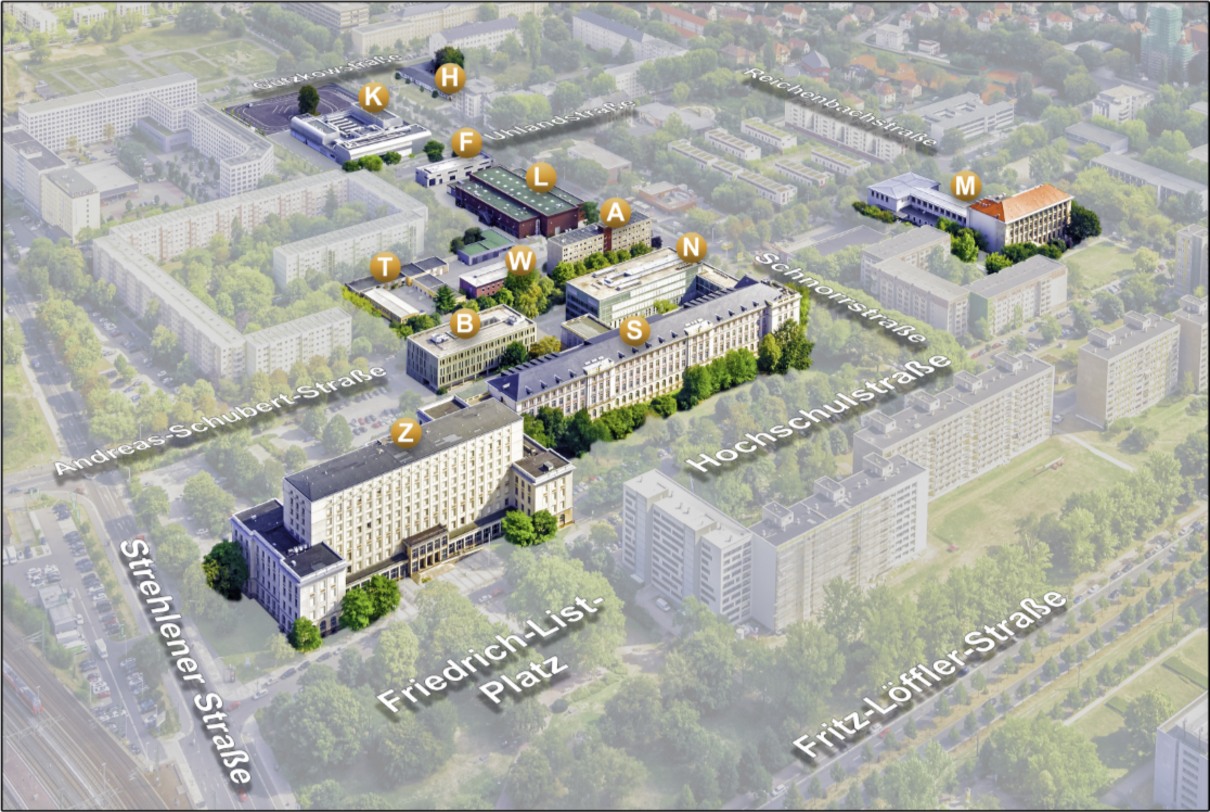
\includegraphics[width=\textwidth]{Bilddatei}
\caption{Bildbeschreibung}
\label{fig:Bildlabel}
\end{figure}

% Endblatt (weiß)
\clearpage
\thispagestyle{empty}
\begin{center}
\vfill
\phantom{© \makeatletter\@author\makeatother}
\end{center}

\end{document}
